\documentclass[12pt,italian,a4paper,oneside,openright]{book}
\usepackage{url,amsfonts,epsfig}
\usepackage[italian]{babel}
\usepackage[latin1]{inputenc}
%\usepackage[format=hang,font=footnotesize]{caption}
\usepackage{amsmath}
\usepackage{indentfirst}
\usepackage{graphicx}
%\usepackage{algorithm,algorithmic}
\graphicspath{{img/}}
\usepackage[hyperindex]{hyperref} %per l'indice interattivo
\hypersetup{colorlinks=true, linkcolor=black} %per colorare i link
\DeclareGraphicsRule{.jpg}{jpg}{}{} %da commentare per il PDF
%\DeclareGraphicsRule{.bmp} {bmp}{}{} %da commentare per il PDF

%%\setmarginsrb{1.5cm}{1.5cm}{1,2cm}{1,5cm}{0cm}{2cm}{2cm}{2cm}


\title{Template per la tesina in .tex}
\author{Nome e Cognome}
\date{Data di esame}

\begin{document}
\pagenumbering{Roman}

%%%% Opzione per interlinea 2
\baselineskip 1.5em

%% FRONTESPIZIO
{ \thispagestyle{empty}


\vskip 1cm \large \centerline{\textsc{Progetto Programmazione 3}}

\begin{center}

\includegraphics[scale=0.50]{logo_parthenope.png}
\end{center}

\vskip 0.5cm

\large \centerline {\textsc{Gestionale - SistemaBancario}}

\vskip 0.5cm

\vskip 4.5cm


\large
\begin{minipage}[t]{7cm}
\textsc{Docente}

\textbf{Prof. Angelo Ciaramella}\newline

\end{minipage}
\hfill
\begin{minipage}[t]{5.5cm}
\textsc{Candidato}

\textbf{Pasquale De Trino}
\textbf{\\Matr. 012400/1637}

\end{minipage}

\vskip 2.0 cm \Large \centerline {Anno Accademico 2018-2019}
\vfill \eject}


%\newpage
%\thispagestyle{plain}
\markboth{Indice}{Indice}
\tableofcontents

\newpage

\pagenumbering{arabic}
\chapter{Descrizione} \label{cap1}
Si richiede di simulare un SistemaBancario per gestire conti correnti e investimenti. \\
Il sistema prevede una doppia modalit\`{a} di accesso, amministratore e utente. \\
In modalit\`{a} amministratore \`{e} possibile, dopo una fase di autenticazione, ricercare un utente tramite id o nome e cognome usando una struttura dati opportuna;
Registrare un utente inserendo dati anagrafici, tipologia di conto corrente saldo della carta prepagata e del conto corrente.
Automaticamente il sistema proprorr\`{a} agli utenti una forma di investimento considerando le caratteristiche dell'utente.

In modalit\`{a} utente \`{e} possibile visualizzare le informazioni sulle operazioni fatte riguardo il proprio conto, fare acquisti tramite una carta,
richiedere l'annullamento dell'ultimo addebito su conto corrente, richiedere uno sconto sugli acquisti tramite un codice sconto, partecipare ad un investimento scegliendo tra quelli disponibili o quello proposto dal sistema.
\chapter{Implementazione} \label{cap2}
\def\baselinestretch{1.66}
Il progetto \`{e} sviluppato in modalit\`{a} Web Application in modo che il software possa risiedere su un server ed essere raggiungibile ed utilizzabile da diversi utenti tramite un comune browser web.\\
\`{E} inoltre possibile in questo modo aggiornare l'applicazione solo sul server e offrire sempre un prodotto aggiornato agli utilizzatori.\\
La web Application pu\`{o} anche essere estesa, \`{e} infatti possibile aggiungere funzionalit\`{a} anche abbastanza complesse poich\`{e}, girando su un server, la potenza dell'hardware \`{e} tale da soddisfare i requisiti tecnici.\\

\section{Web Aplication}
I principali vantaggi di una web application riguardano le possibilit\`{a} di utilizzare l'applicazione senza problemi di compatibilit\`{a} di versione di Java oppure di dipendenze da software esterni quali ad esempio DBMS o particolari librerie grafiche.\\
\section{Web Server}
Il Web Server si occupa di predisporre e restituire le pagine web al client.\\
L'Applicaton Server si occupa di gestire la logica applicativa e interfacciarsi con altri moduli. \\
Talvolta i ruoli sono fusi in un unico oggetto, definito Web Container,\\ Tomcat ne \`{e} un esempio.\\
\subsection{Servlets}
Le servlets sono classi Java che consentono l'interazione richiesta/risposta secondo il modello client/server utilizzando i metodi doGet e doPost.\\
Il pattern MVC (Model View Controller), consente di separare la logica di presentazione da quella di business.\\
Utilizzando le servlets \`{e} possibile congiungere le due logiche scambiando informazioni utilizzando i metodi estesi dalla classe HttpServlet.



\chapter{Descrizione UML} \label{cap}
\def\baselinestretch{1.66}

Seguendo il diagramma UML delle classi spieghiamo come \`{e} stato sviluppato il software.\\

\section{Factory Pattern}
L'accesso pu\`{o} avvenire in modalit\`{a} utente o in modalit\`{a} amministratore, a tal proposito \`{e} stato utilizzato un \textbf{factory pattern}, il metodo Accedi della classe Login \`{e} implementato dalle classi Utente e Amministratore per controllare le credenziali di accesso in due differenti tabelle. \\
\begin{center}
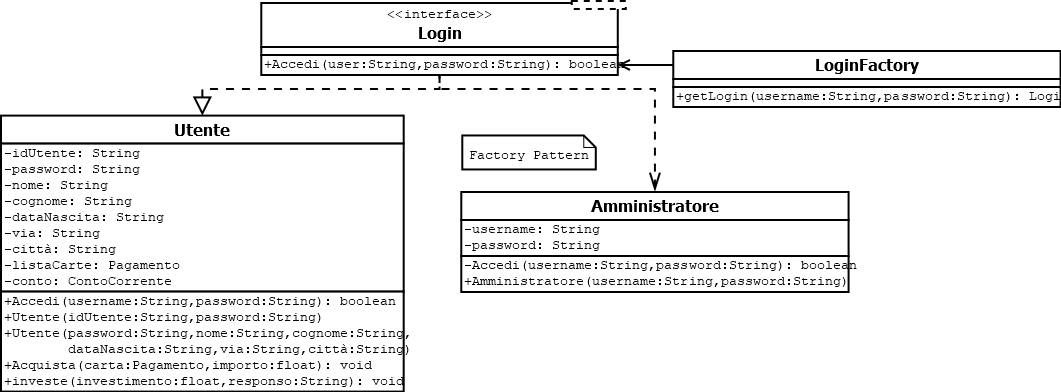
\includegraphics[scale=0.40]{FactoryPattern.png}
\end{center}

\section{Chain of Responsibility}
Proseguendo la lettura del diagramma in direzione dell'Amministratore, il pattern \textbf{CoR} definisce una classe astratta Investimento e le classi concrete BassoRischio, MedioRischio e AltoRischio che applicano una diversa logica al metodo investi.\\
La conclusione del pattern \`{e} nella servlet EffettuaInvestimento che data una stringa da alla prima classe della catena la richiesta che seguir\`{a} poi fino a trovare chi pu\`{o} soddisfare la richiesta. \\
\begin{center}
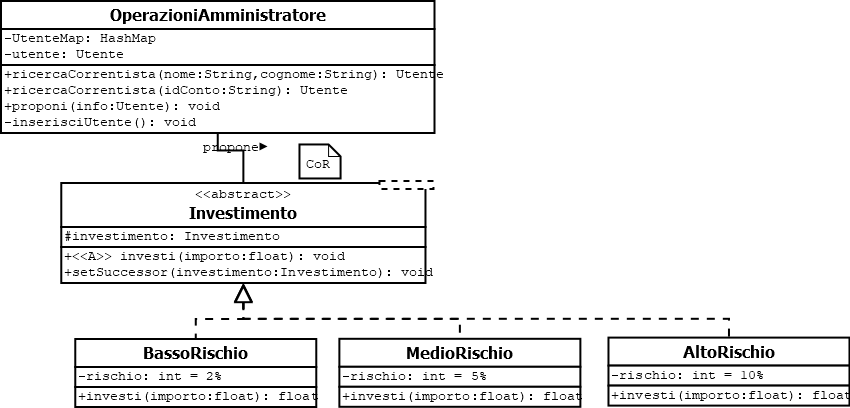
\includegraphics[scale=0.40]{CoR.png}
\end{center}

\section{Template Method}
Passando alla parte dello schema riguardante l' utente, il primo pattern \`{e} \textbf{TemplateMethod} il quale \`{e} stato pensato per astrarre il comportamento dei metodi versa e preleva che sono implementati dalle classi ContoBasic, ContoMedium, ContoPremium fornendo l'implementazione dei restanti metodi che risulteranno comuni per i vari tipi di conto corrente.\\
\begin{center}
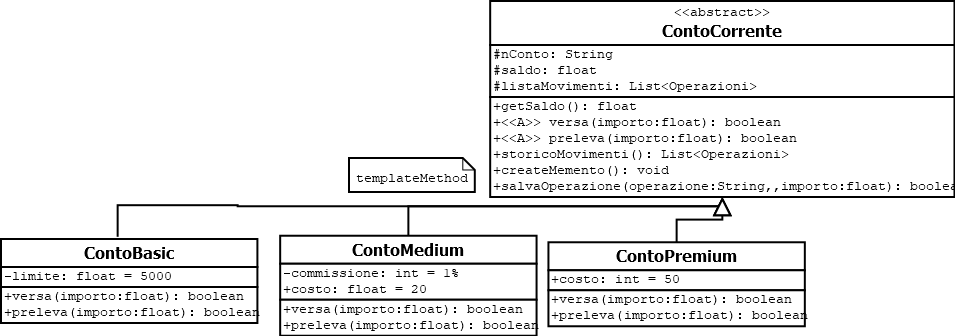
\includegraphics[scale=0.40]{TemplateMethod.png}
\end{center}

\section{Memento}
Il pattern \textbf{Memento} permette all'utente di poter annullare l'ultimo \\ acquisto effettuato tramite carta di credito. \\
\begin{center}
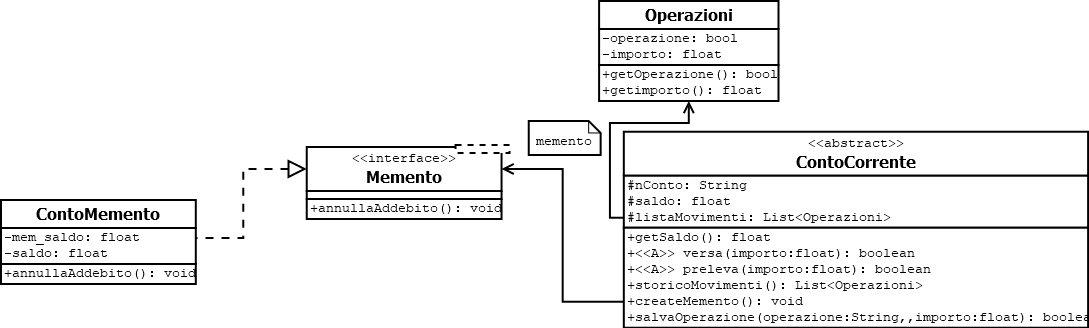
\includegraphics[scale=0.40]{Memento.png}
\end{center}

\section{Strategy}
L' utente pu\`{o} effettuare un acquisto con carta di credito o con carta prepagata, il pattern \textbf{strategy} consente di implementare due strategie di pagamento differenti, nel primo caso viene applicata la logica di pagamento relativa al tipo di conto corrente posseduto, nel secondo controllando il saldo della carta prepagata.\\
\begin{center}
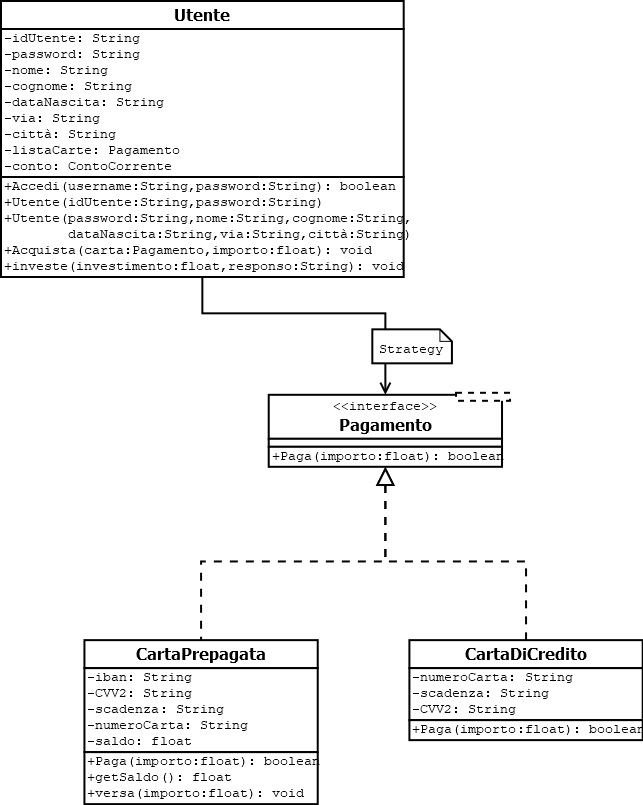
\includegraphics[scale=0.40]{Strategy.png}
\end{center}
\newpage
\section{Decorator}
La possibilit\`{a} di aggiungere uno sconto a run-time al proprio conto corrente \`{e} realizzata mediante il pattern \textbf{decorator}. In base al codice sconto iserito, l'utente riceve un diverso tipo di codice sconto, viene dunque decorato l'oggetto relativo al proprio conto corrente.\\
\begin{center}
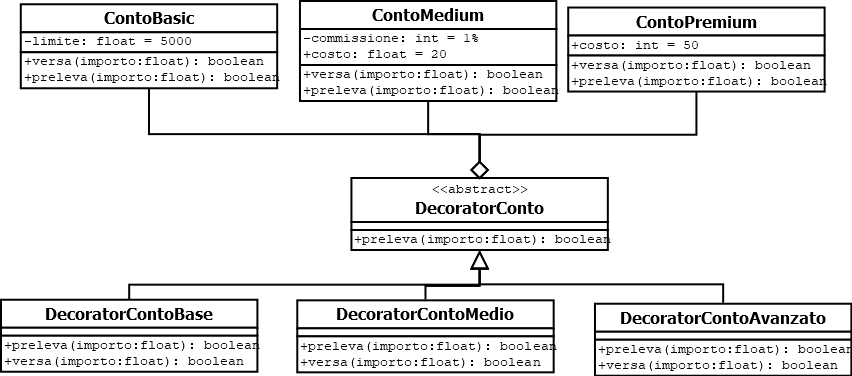
\includegraphics[scale=0.40]{Decorator.png}
\end{center}

Il pattern \textbf{singleton} \`{e} usato in diversi contesti per mantenere un unica istanza degli oggetti discendenti da contoCorrente, in modo che essi possano essere eventualmente decorati.\\

 

\newpage
\pagestyle{plain}

%\input{tesi_tex/ringraziamenti.tex}

\end{document}
